\chapter{HASIL DAN PENGUJIAN}
\label{chap:hasildanpengujian}

% Ubah bagian-bagian berikut dengan isi dari pengujian dan analisis

Dalam bab ini, penulis menyajikan hasil-hasil yang diperoleh dari penelitian
ini. Penelitian yang dilakukan bertujuan untuk mencapai pemahaman yang lebih
mendalam mengenai aspek-aspek yang relevan dengan topik yang dibahas. Hasil
yang diharapkan dari penelitian ini adalah untuk memberikan wawasan baru yang
bermanfaat dalam konteks yang sedang diteliti, serta untuk memvalidasi atau
memperbarui pengetahuan yang sudah ada. Dengan mengacu pada tujuan penelitian,
diharapkan temuan-temuan ini dapat memberikan kontribusi yang signifikan
terhadap pemecahan masalah yang dihadapi dalam domain penelitian yang terkait.

\section{Hasil}
\label{sec:hasil}

\begin{figure}[H]
  \centering
  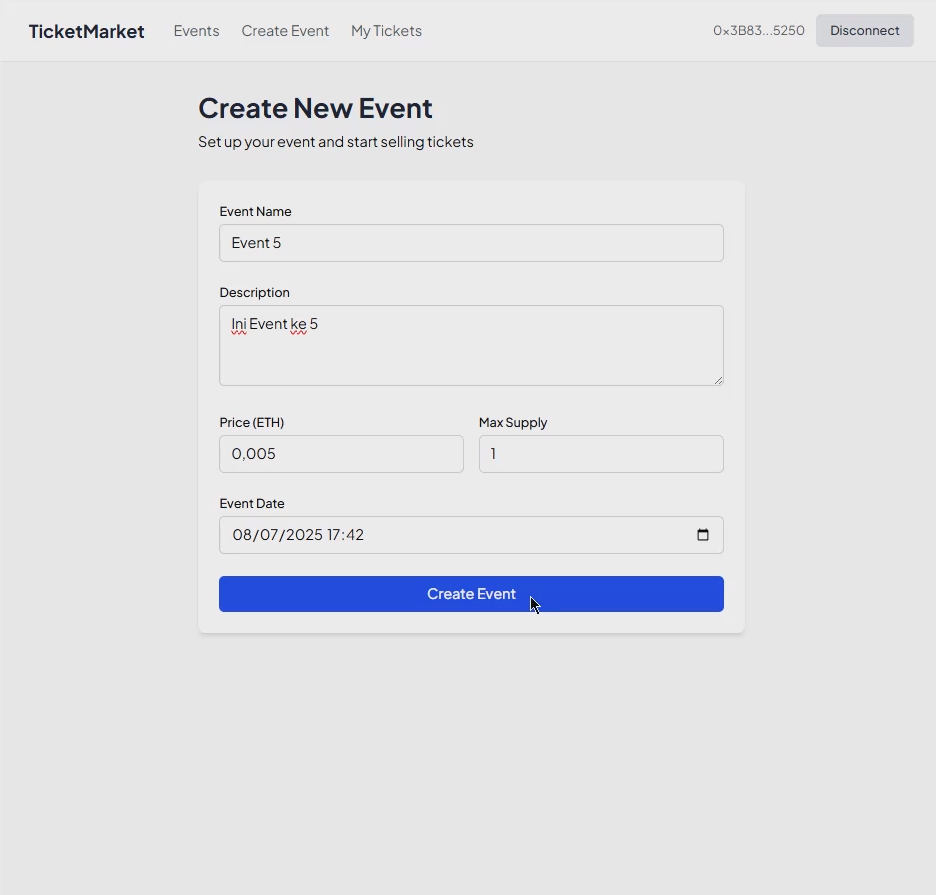
\includegraphics[width=0.75\textwidth]{gambar/bab4/create-new-event.png}
  \caption{Formulir Pembuatan Event Baru}
  \label{fig:create-new-event}
\end{figure}
Gambar \ref{fig:create-new-event} menunjukkan antarmuka pengguna untuk
membuat event baru pada \emph{platform marketplace} tiket konser berbasis \emph{smart
  contract}. Formulir ini memungkinkan pengguna untuk memasukkan informasi
penting seperti nama event, tanggal, waktu, dan jumlah tiket yang
tersedia. Setelah mengisi formulir, pengguna dapat menekan tombol
\emph{Create Event} untuk mengirimkan data ke \emph{smart contract} yang
telah di-deploy pada jaringan Layer-2 Ethereum, yaitu \emph{Polygon zkEVM}.
Proses ini akan menghasilkan transaksi yang menciptakan event baru pada
blockchain, yang kemudian dapat dilihat pada \emph{block explorer} seperti
\emph{PolygonScan}. Dengan demikian, pengguna dapat dengan mudah membuat event
baru dan mengelola tiket konser secara terdesentralisasi, aman, dan transparan.
\begin{figure}[H]
  \centering
  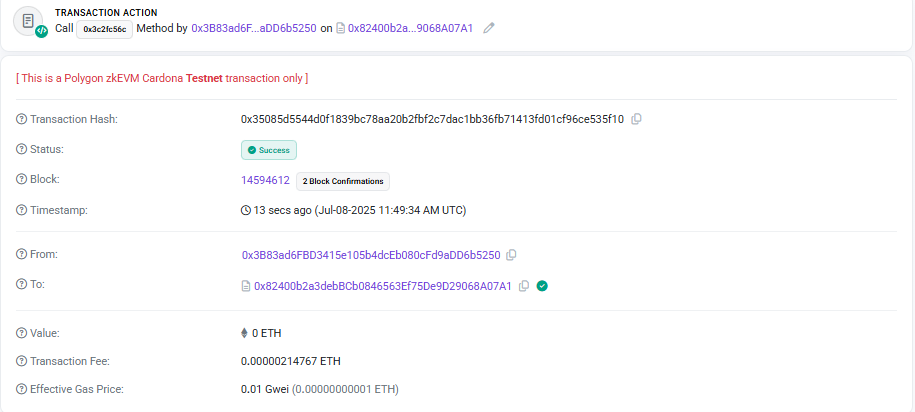
\includegraphics[width=\textwidth]{gambar/bab4/Screenshot 2025-07-08 185014.png}
  \caption{Bukti Transaksi Pembuatan Event Baru}
  \label{fig:biaya-pembuatan-event}
\end{figure}
Dapat dilihat pada \emph{Block Explorer} bahwa \emph{createEvent} membutuhkan biaya transaksi sebesar\textbf{0.000002147867 ETH} dan biaya gas yang dikeluarkan
adalah \textbf{0.01 Gwei}. Durasi transaksi terjadi selama \textbf{13 detik} dengan \textbf{2 \emph{block confirmations}}.
\begin{figure}[H]
  \centering
  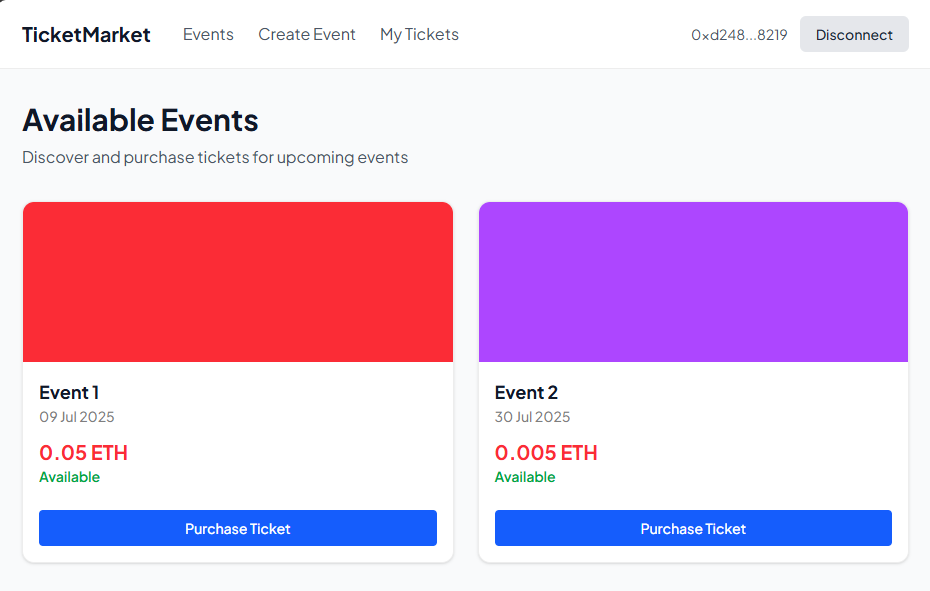
\includegraphics[width=.75\textwidth]{gambar/bab4/Screenshot 2025-07-08 200947.png}
  \caption{Halaman Event yang Dibuat}
  \label{fig:halaman-event-dibuat}
\end{figure}

Gambar \ref{fig:halaman-event-dibuat} menunjukkan halaman event yang telah
dibuat. Halaman ini menampilkan informasi penting mengenai event, seperti nama
event, tanggal, waktu, dan jumlah tiket yang tersedia. Pengguna dapat melihat
detail event dan melakukan pembelian tiket dengan menekan tombol \emph{Purchase
  Ticket}. Setelah menekan tombol tersebut, pengguna akan diarahkan ke halaman
pembelian tiket yang memungkinkan mereka untuk memilih jumlah tiket yang ingin
dibeli. Halaman ini juga menampilkan informasi mengenai harga tiket dan total
biaya yang haruss dibayar. Dengan demikian, pengguna dapat dengan mudah
mengakses informasi mengenai event yang telah dibuat dan melakukan pembelian
tiket secara langsung melalui antarmuka pengguna yang telah disediakan.

\begin{figure}[H]
  \centering
  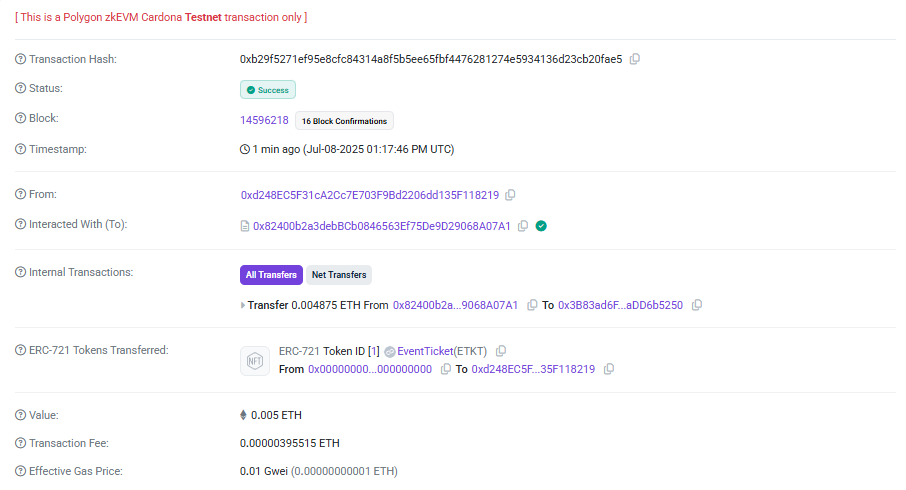
\includegraphics[width=.75\textwidth]{gambar/bab4/Screenshot 2025-07-08 201903.png}
  \caption{Bukti pembelian tiket pada event yang telah dibuat}
  \label{fig:bukti-pembelian-tiket}

\end{figure}
Gambar \ref{fig:bukti-pembelian-tiket} menunjukkan ticket minting process dimana event organizers men-create NFT ticket baru dan mentransfernya kepada purchaser, dengan remarkably low transaction fee sebesar \textbf{0.000003955515 ETH} dan effective gas price \textbf{0.01 Gwei}.

\begin{figure}[H]
  \centering
  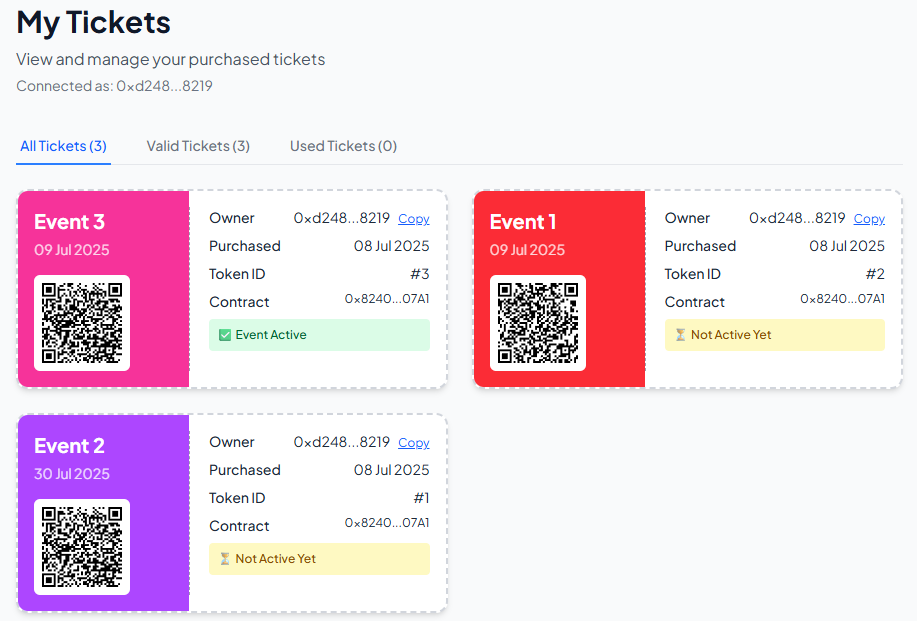
\includegraphics[width=.85\textwidth]{gambar/bab4/Screenshot 2025-07-08 215504.png}
  \caption{Halaman tiket yang telah dibeli}
  \label{fig:halaman-tiket-dibeli}
\end{figure}

Gambar \ref{fig:halaman-tiket-dibeli} menunjukkan halaman tiket yang telah
dibeli. Halaman ini menampilkan informasi penting mengenai tiket, seperti nama
event, tanggal, waktu, dan jumlah tiket yang telah dibeli. Pengguna juga dapat
melihat detail tiket yang telah dibeli, termasuk nomor tiket, harga, dan status
tiket. Pembeli juga dapat menverifikasi kesabsahan tiket dengan melihat alamat
NFT ke Block Explorer.

\begin{figure}[H]
  \centering
  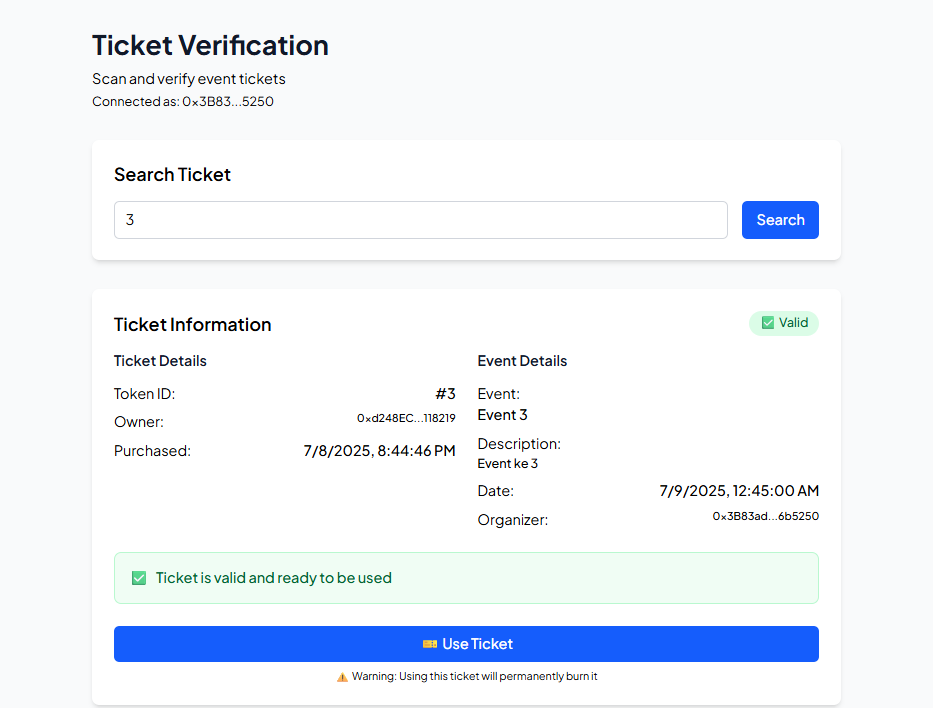
\includegraphics[width=.65\textwidth]{gambar/bab4/Screenshot 2025-07-08 204651.png}
  \caption{Halaman verifikasi tiket yang telah dibeli}
  \label{fig:halaman-verifikasi-tiket}
\end{figure}
Gambar \ref{fig:halaman-verifikasi-tiket} menunjukkan halaman verifikasi
tiket yang telah dibeli. Halaman ini hanya dapat diakses oleh pembuat event
yang telah membuat event sebelumnya. Halaman ini menampilkan informasi penting
mengenai tiket yang telah dibeli, seperti nama event, tanggal, waktu, dan jumlah
tiket yang telah dibeli. Pada bagian bawah terdapat tombol \emph{Use Ticket} yang berfungsi untuk
menggunakan tiket yang telah dibeli yang dioperasikan oleh pembuat tiket. Setelah menekan tombol tersebut, tiket akan
ditandai sebagai telah digunakan dan tidak dapat digunakan kembali.

\section{Pengujian Pada Jaringan Ethereum, Polygon zkEVM, dan Polygon POS}
Pengujian dilakukan pada tiga jaringan blockchain yang berbeda yaitu Ethereum
Sepolia Testnet, Polygon zkEVM Cardona Testnet, dan Polygon POS Amoy Testnet.
Tujuan dari pengujian ini adalah untuk menganalisis performa dan efisiensi dari
\emph{smart contract} yang telah di-deploy pada masing-masing jaringan.
Pengujian dilakukan dengan menggunakan \emph{smart contract} yang sama pada
ketiga jaringan untuk memastikan perbandingan yang adil. Setiap jaringan
memiliki karakteristik yang berbeda dalam hal kecepatan, biaya transaksi, dan
kapasitas pemrosesan. Pengujian berdasarkan fungsionalitas utama dari
\emph{smart contract} yaitu pembuatan event, pembelian tiket, dan penggunaan
tiket.

\subsection{Pengujian Perilisan \emph{Smart Contract} Pada Jaringan Blockchain}
\begin{table}[h]
  \centering
  \begin{tabular}{|c|c|c|c|c|}
    \hline
    \textbf{Network} & \textbf{Gas Used} & \textbf{Gas Price (Gwei)} & \textbf{Cost} & \textbf{Time (s)} \\
    \hline
    Cardona          & 5,251,898         & 0.01                      & 0.0000525 ETH & 13.20             \\
    Amoy             & 5,253,460         & 37.57                     & 0.1974 POL    & 5.84              \\
    Sepolia          & 5,253,460         & 21.77                     & 0.0001144 ETH & 8.72              \\
    \hline
  \end{tabular}
  \caption{Hasil Pengujian Perilisan \emph{Smart Contract}}
\end{table}

Performa deployment kontrak menunjukkan perbedaan karakteristik fundamental
dari setiap jaringan dalam menangani transaksi kompleks. Ketiga jaringan
menggunakan gas yang hampir identik untuk deployment (sekitar 5.25 juta gas),
yang mengkonfirmasi bahwa kompleksitas komputasi \emph{smart contract} adalah
sama terlepas dari jaringan yang digunakan. Perbedaan utama terletak pada gas
price dan waktu eksekusi yang mencerminkan kondisi jaringan dan implementasi
teknologi yang berbeda. Cardona zkEVM menunjukkan gas price terendah yaitu 0.01
Gwei, yang menghasilkan biaya deployment hanya 0.0000525 ETH. Hal ini
mencerminkan strategi Polygon untuk menjadikan zkEVM sebagai solusi yang
cost-effective bagi developer. Namun, waktu deployment yang paling lama (13.20
detik) mengindikasikan bahwa teknologi zero-knowledge proof masih memerlukan
waktu komputasi tambahan untuk memproses dan memverifikasi transaksi, yang
merupakan trade-off alami dari keamanan dan skalabilitas yang ditawarkan.
Jaringan Amoy menunjukkan performa tercepat dengan waktu deployment hanya 5.84
detik, membuktikan kematangan infrastruktur Polygon sebagai layer-2 solution.
Namun, gas price yang tinggi sebesar 37.57 Gwei mengakibatkan biaya deployment
yang paling mahal yaitu 0.1974 POL. Kecepatan ini dicapai melalui mekanisme
konsensus Proof-of-Stake yang efficient dan infrastruktur node yang
terdistribusi dengan baik di seluruh jaringan. Sepolia sebagai testnet Ethereum
menunjukkan performa yang berada di tengah-tengah dengan gas price 21.77 Gwei
dan waktu deployment 8.72 detik. Biaya deployment sebesar 0.0001144 ETH
mencerminkan kondisi jaringan Ethereum yang stabil namun tidak seoptimal
layer-2 solutions dalam hal kecepatan. Waktu deployment yang moderat ini
konsisten dengan karakteristik Ethereum yang mengutamakan security dan
decentralization dibandingkan speed. Analisis komparatif menunjukkan bahwa
pemilihan jaringan untuk deployment harus mempertimbangkan prioritas aplikasi.
Untuk aplikasi yang mengutamakan cost-efficiency, Cardona menjadi pilihan
optimal meskipun dengan waktu deployment yang lebih lama. Untuk aplikasi yang
memerlukan deployment cepat dan ready-to-use, Amoy memberikan solusi terbaik
meskipun dengan biaya yang lebih tinggi. Sementara Sepolia cocok untuk testing
yang memerlukan kondisi mendekati mainnet Ethereum dengan biaya dan waktu yang
reasonable.

\subsection{Pengujian Pembuatan Tiket Konser}

\begin{table}[h]
  \centering
  \begin{tabular}{|c|c|c|c|c|}
    \hline
    \textbf{Network} & \textbf{Gas Used} & \textbf{Gas Price (Gwei)} & \textbf{Cost}  & \textbf{Time (s)} \\
    \hline
    Cardona          & 276,965           & 0.01                      & 0.00000277 ETH & 8.88              \\
    Amoy             & 276,965           & 37.54                     & 0.01040 POL    & 4.19              \\
    Sepolia          & 276,965           & 21.90                     & 0.00000607 ETH & 11.02             \\
    \hline
  \end{tabular}
  \caption{Hasil Pengujian Pembuatan Tiket Konser}
\end{table}
Performa pembuatan event menunjukkan konsistensi yang menarik dalam hal penggunaan gas di ketiga jaringan, dengan semua menggunakan tepat 276,965 gas. Konsistensi ini mengkonfirmasi bahwa fungsi createEvent dalam \emph{smart contract} Ticket Marketplace telah dioptimasi dengan baik dan menghasilkan bytecode yang efficient. Perbedaan performa utama kembali terletak pada gas price dan execution time, yang mencerminkan karakteristik infrastruktural masing-masing jaringan.
Cardona kembali menunjukkan keunggulan dalam hal cost-effectiveness dengan gas price 0.01 Gwei yang menghasilkan biaya hanya 0.00000277 ETH untuk pembuatan event. Waktu eksekusi 8.88 detik menunjukkan peningkatan performa dibandingkan deployment, mengindikasikan bahwa transaksi yang lebih sederhana dapat diproses lebih efisien oleh zkEVM. Hal ini memberikan optimisme bahwa operasi-operasi rutin dalam aplikasi marketplace dapat berjalan dengan lancar dan cost-effective di jaringan ini.
Amoy mempertahankan posisinya sebagai jaringan tercepat dengan waktu eksekusi hanya 4.19 detik, hampir separuh dari waktu yang dibutuhkan Cardona. Kecepatan ini sangat menguntungkan untuk user experience, terutama dalam aplikasi marketplace dimana responsivitas adalah kunci kepuasan pengguna. Namun, biaya 0.01040 POL yang dihasilkan dari gas price 37.54 Gwei menunjukkan trade-off yang signifikan antara speed dan cost.
Sepolia menunjukkan waktu eksekusi terlama yaitu 11.02 detik untuk pembuatan event, yang bahkan lebih lama dari deployment ratio-wise. Hal ini mengindikasikan bahwa jaringan Ethereum testnet mungkin mengalami congestion atau memiliki block time yang lebih konservatif. Gas price 21.90 Gwei menghasilkan biaya 0.00000607 ETH, yang masih reasonable dan kompetitif dibandingkan dengan Amoy.
Implikasi bisnis dari data ini sangat relevan untuk aplikasi marketplace. Untuk event organizer yang sering membuat event dalam volume besar, perbedaan biaya dan waktu ini dapat menjadi faktor decisive. Cardona menawarkan solusi yang sustainable untuk operasi skala besar dengan biaya minimal, sementara Amoy memberikan user experience terbaik untuk aplikasi yang mengutamakan real-time responsiveness. Sepolia memberikan testing environment yang reliable untuk validasi sebelum deployment ke mainnet.

\subsection{Pengujian Pembelian Tiket Konser}
\begin{table}[h]
  \centering
  \begin{tabular}{|c|c|c|c|c|c|}
    \hline
    \textbf{Network} & \textbf{Ticket \#} & \textbf{Gas Used} & \textbf{Gas Price (Gwei)} & \textbf{Cost}  & \textbf{Time (s)} \\
    \hline
    \multirow{5}{*}{Cardona (ETH)}
                     & 1                  & 392,907           & 0.01                      & 0.00000393 ETH & 8.84              \\
                     & 2                  & 307,407           & 0.01                      & 0.00000307 ETH & 8.82              \\
                     & 3                  & 307,407           & 0.01                      & 0.00000307 ETH & 9.26              \\
                     & 4                  & 307,407           & 0.01                      & 0.00000307 ETH & 8.96              \\
                     & 5                  & 307,407           & 0.01                      & 0.00000307 ETH & 9.56              \\
    \hline
    \multirow{5}{*}{Amoy (POL)}
                     & 1                  & 392,907           & 37.54                     & 0.01475 POL    & 2.31              \\
                     & 2                  & 307,407           & 37.54                     & 0.01154 POL    & 4.23              \\
                     & 3                  & 307,407           & 37.54                     & 0.01154 POL    & 6.79              \\
                     & 4                  & 307,407           & 37.54                     & 0.01154 POL    & 3.82              \\
                     & 5                  & 307,407           & 41.57                     & 0.01278 POL    & 3.04              \\
    \hline
    \multirow{5}{*}{Sepolia (ETH)}
                     & 1                  & 392,907           & 22.11                     & 0.00000869 ETH & 12.08             \\
                     & 2                  & 307,407           & 23.78                     & 0.00000731 ETH & 12.45             \\
                     & 3                  & 307,407           & 23.68                     & 0.00000728 ETH & 10.63             \\
                     & 4                  & 307,407           & 23.29                     & 0.00000716 ETH & 13.30             \\
                     & 5                  & 307,407           & 24.03                     & 0.00000739 ETH & 11.07             \\
    \hline
  \end{tabular}
  \caption{Hasil Pengujian Pembelian Tiket Konser}
\end{table}

Analisis detail performa pembelian tiket individual memberikan granular insight
tentang consistency dan predictability setiap jaringan. Pola yang menarik
terlihat dari perbedaan gas usage antara ticket pertama dan subsequent tickets,
dimana ticket pertama selalu menggunakan gas lebih tinggi (392,907 gas)
dibandingkan tickets berikutnya (307,407 gas). Pola ini konsisten di semua
jaringan dan mencerminkan \emph{smart contract} optimization dimana state
initialization memerlukan gas tambahan, sementara subsequent operations dapat
memanfaatkan cached state. Pada Cardona, consistency dalam gas price 0.01 Gwei
di semua transaksi menunjukkan stability jaringan yang baik. Waktu transaksi
berkisar antara 8.82 hingga 9.56 detik dengan variasi yang minimal,
mengindikasikan predictable performance yang valuable untuk user experience
planning. Cost consistency dengan rentang 0.00000307 ETH untuk tickets 2-5
memberikan transparency dalam operational cost calculation. Amoy menunjukkan
variabilitas yang lebih tinggi dalam waktu transaksi, dari 2.31 detik hingga
6.79 detik, yang mungkin mencerminkan network condition fluctuation atau load
balancing mechanism. Menariknya, ticket terakhir menggunakan gas price yang
lebih tinggi (41.57 Gwei vs 37.54 Gwei), yang mengindikasikan dynamic gas
pricing mechanism yang responsive terhadap network congestion. Kecepatan
tercepat 2.31 detik pada ticket pertama menunjukkan potential optimal
performance jaringan ini. Sepolia menunjukkan variabilitas gas price yang
paling tinggi, berkisar dari 22.11 hingga 24.03 Gwei, yang mencerminkan
market-driven gas pricing mechanism yang typical pada Ethereum ecosystem. Waktu
transaksi yang bervariasi dari 10.63 hingga 13.30 detik menunjukkan dependency
terhadap network congestion dan block inclusion priority. Variabilitas ini
memberikan realistic preview tentang kondisi yang akan dihadapi pada Ethereum
mainnet. Pattern analysis menunjukkan bahwa untuk aplikasi production,
understanding terhadap gas usage pattern ini crucial untuk cost optimization.
\emph{Smart contract} dapat dioptimasi lebih lanjut untuk mengurangi gas
overhead pada transaksi pertama, atau mengimplementasi batch processing untuk
multiple ticket purchases. Network selection juga harus consider tidak hanya
average performance, tetapi juga variability dan predictability, yang dapat
significantly impact user experience dalam kondisi real-world usage dengan
various network conditions dan traffic patterns.

\section{Pengujian Kinerja Pada \emph{Smart Contract}}
Terdapat 10 skenario pengujian yang digunakan untuk menguji \emph{Smart Contract}

\subsection{Skenario Uji Performa untuk Peningkatan Pembelian}
\begin{table}[h!]
  \centering
  \begin{tabular}{|c|c|c|c|c|c|c|}
    \hline
    \textbf{Step} & \textbf{Concurrent}   & \textbf{Total Tx} & \textbf{Avg Gas} & \textbf{Avg Response} & \textbf{TPS} & \textbf{Peak TPS} \\
    \textbf{}     & \textbf{Transactions} & \textbf{}         & \textbf{Used}    & \textbf{Time (ms)}    & \textbf{}    & \textbf{}         \\
    \hline
    1             & 2                     & 10                & 346,299          & 12.9                  & 0.99         & 200.0             \\
    \hline
    2             & 4                     & 20                & 337,749          & 18.3                  & 1.98         & 285.7             \\
    \hline
    3             & 6                     & 30                & 336,039          & 29.5                  & 2.95         & 285.7             \\
    \hline
    4             & 8                     & 40                & 335,184          & 39.7                  & 3.91         & 228.6             \\
    \hline
    5             & 10                    & 50                & 334,671          & 46.7                  & 4.65         & 227.3             \\
    \hline
  \end{tabular}
  \caption{Hasil Pengujian Performa Ramp-Up Pembelian pada Jaringan Cardona}
  \label{tab:cardona_performance}
\end{table}

Hasil pengujian ramp-up pada jaringan Cardona menunjukkan karakteristik
performa yang sangat mengesankan dan konsisten sepanjang lima tahap peningkatan
beban transaksi secara bertahap. Dari data yang tercatat, dapat diamati bahwa
jaringan Cardona mampu mempertahankan tingkat keberhasilan transaksi yang
sempurna sebesar 100\% di seluruh tahap pengujian, mulai dari beban ringan
dengan 2 transaksi konkuren hingga beban yang lebih intensif dengan 10
transaksi konkuren. Pola peningkatan throughput yang linear terlihat jelas
dimana transactions per second (TPS) meningkat secara proporsional dengan
jumlah transaksi konkuren, dari 0.99 TPS pada tahap pertama hingga mencapai
4.65 TPS pada tahap kelima, menunjukkan bahwa jaringan Cardona memiliki
kemampuan scaling yang baik dalam menangani peningkatan beban kerja. Aspek yang
menarik dari hasil ini adalah stabilitas penggunaan gas yang relatif konsisten
di seluruh tahap testing, dengan rata-rata gas usage berkisar antara 334,671
hingga 346,299 gas per transaksi. Variasi gas usage yang minimal ini
menunjukkan bahwa kompleksitas komputasi untuk operasi pembelian tiket tidak
terpengaruh secara signifikan oleh tingkat konkurensi, mengindikasikan
efisiensi algoritma konsensus dan execution layer jaringan Cardona. Namun
demikian, terdapat tren peningkatan waktu respons yang gradual seiring dengan
peningkatan beban, dimana average response time meningkat dari 12.9 milidetik
pada tahap pertama menjadi 46.7 milidetik pada tahap kelima. Peningkatan ini
masih dalam batas yang sangat reasonable untuk aplikasi blockchain, mengingat
bahwa bahkan pada beban tertinggi, waktu respons masih berada di bawah 50
milidetik, yang jauh lebih cepat dibandingkan dengan standar industri untuk
aplikasi decentralized. Peak TPS yang dicapai dalam pengujian ini mencapai
titik tertinggi pada tahap kedua dan ketiga dengan 285.7 TPS, menunjukkan bahwa
jaringan Cardona memiliki kapasitas burst yang sangat tinggi untuk menangani
lonjakan transaksi dalam periode waktu singkat. Meskipun peak TPS mengalami
sedikit penurunan pada tahap keempat dan kelima menjadi sekitar 227-228 TPS,
nilai ini tetap menunjukkan performa yang luar biasa dibandingkan dengan
jaringan blockchain lainnya. Konsistensi performa yang tinggi ini
mengindikasikan bahwa jaringan Cardona telah dioptimasi dengan baik untuk
menangani workload yang bervariasi tanpa mengalami degradasi performa yang
signifikan, menjadikannya platform yang sangat suitable untuk aplikasi
marketplace NFT yang memerlukan throughput tinggi dan response time yang
konsisten.

\begin{table}[h!]
  \centering
  \begin{tabular}{|c|c|c|c|c|}
    \hline
    \textbf{Step} & \textbf{Peak TPS} & \textbf{Min TPS} & \textbf{Average TPS} & \textbf{Consistency Score} \\
    \hline
    1             & 200.0             & 117.6            & 152.0                & 100                        \\
    \hline
    2             & 285.7             & 148.1            & 220.9                & 100                        \\
    \hline
    3             & 285.7             & 127.7            & 207.8                & 100                        \\
    \hline
    4             & 228.6             & 109.6            & 193.8                & 100                        \\
    \hline
    5             & 227.3             & 175.4            & 200.1                & 100                        \\
    \hline
  \end{tabular}
  \caption{Ringkasan Metrik Performa}
  \label{tab:performance_metrics}
\end{table}

Analisis terhadap performance metrics summary mengungkapkan karakteristik
mendasar dari jaringan Cardona dalam hal skalabilitas, konsistensi, dan
kapabilitas kinerja puncak yang sangat mengesankan, terlebih untuk ukuran
sebuah jaringan testnet blockchain. Nilai Peak TPS (transaction per second
tertinggi) menunjukkan pola yang menarik, di mana performa tertinggi sebesar
285,7 TPS tercapai pada tahap kedua dan ketiga (dengan 4 dan 6 transaksi yang
berjalan secara bersamaan), kemudian mengalami penurunan secara bertahap
menjadi sekitar 227–228 TPS pada tahap keempat dan kelima (dengan 8 dan 10
transaksi bersamaan). Pola ini mengindikasikan adanya level optimal untuk
concurrent transactions pada jaringan Cardona, yakni pada kisaran 4–6 transaksi
bersamaan. Setelah melewati ambang ini, penambahan beban tidak lagi
menghasilkan peningkatan performa secara linier, melainkan menunjukkan efek
diminishing returns yang kemungkinan disebabkan oleh kontensi sumber daya
(resource contention) atau meningkatnya beban koordinasi (coordination
overhead). Nilai Minimum TPS yang tercatat pada tiap tahap pengujian memberikan
gambaran tentang performa dasar jaringan dalam kondisi terburuk. Rentang nilai
minimum TPS yang relatif stabil antara 109 hingga 175 TPS menunjukkan bahwa
bahkan dalam kondisi beban tinggi atau skenario ekstrem, jaringan masih mampu
mempertahankan throughput yang cukup tinggi dan layak. Hal yang patut dicatat
adalah bahwa selisih antara nilai minimum dan puncak TPS tidak menunjukkan
kecenderungan untuk melebar secara drastis seiring dengan meningkatnya beban
transaksi, yang berarti variansi performa tetap terkontrol dengan baik meskipun
dalam kondisi stres yang lebih tinggi. Hal ini menandakan bahwa algoritma
scheduling dan manajemen sumber daya dalam jaringan Cardona telah dioptimalkan
untuk meminimalkan fluktuasi performa.

Nilai Average TPS yang konsisten berada dalam kisaran 152 hingga 220 TPS
menunjukkan kemampuan performa berkelanjutan (sustained performance) yang
sangat baik dan dapat diandalkan untuk keperluan aplikasi produksi. Tren
Average TPS yang meningkat dari 152 TPS pada tahap pertama ke puncaknya di
tahap kedua (220,9 TPS), lalu relatif stabil dengan sedikit penurunan pada
tahap-tahap selanjutnya, memperkuat dugaan bahwa titik operasi optimal jaringan
Cardona berada pada tingkat beban menengah. Sementara itu, skor konsistensi
(Consistency Score) yang sempurna, yakni 100\% di seluruh tahap pengujian,
merupakan pencapaian luar biasa. Hal ini menunjukkan bahwa standar deviasi dari
tingkat keberhasilan transaksi adalah nol—dengan kata lain, tidak ada
variabilitas dalam tingkat keberhasilan transaksi di antara berbagai batch
dalam setiap fase pengujian. Skor konsistensi yang sempurna ini menunjukkan
bahwa jaringan Cardona memiliki mekanisme pemrosesan transaksi yang sangat
andal dan tidak terpengaruh oleh perubahan kondisi beban. Oleh karena itu,
jaringan ini sangat layak digunakan untuk aplikasi-aplikasi kritikal
(mission-critical applications) yang membutuhkan eksekusi transaksi yang dapat
diprediksi dan sangat andal.

\begin{table}[h!]
  \centering
  \begin{tabular}{|c|c|c|c|c|}
    \hline
    \textbf{Step} & \textbf{First Batch} & \textbf{Subsequent Batches} & \textbf{Gas Difference} & \textbf{Percentage Difference} \\
    \textbf{}     & \textbf{Avg Gas}     & \textbf{Avg Gas}            & \textbf{}               & \textbf{(\%)}                  \\
    \hline
    1             & 401,019              & 332,619                     & 68,400                  & 20.6                           \\
    \hline
    2             & 358,269              & 332,619                     & 25,650                  & 7.7                            \\
    \hline
    3             & 349,719              & 332,619                     & 17,100                  & 5.1                            \\
    \hline
    4             & 345,444              & 332,619                     & 12,825                  & 3.9                            \\
    \hline
    5             & 342,879              & 332,619                     & 10,260                  & 3.1                            \\
    \hline
  \end{tabular}
  \caption{Analisis Penggunaan Gas Berdasarkan Jenis Transaksi}
  \label{tab:gas_analysis}
\end{table}
Analisis penggunaan gas berdasarkan tipe transaksi mengungkapkan pola yang sangat signifikan dan konsisten di seluruh fase pengujian. Ditemukan adanya perbedaan konsumsi gas yang cukup mencolok antara batch pertama dengan batch–batch berikutnya pada setiap tahap pengujian. Fenomena ini menunjukkan adanya beban inisialisasi state yang cukup besar di awal setiap fase pengujian, di mana batch pertama secara konsisten mengonsumsi gas dalam jumlah yang lebih tinggi dengan selisih yang cukup signifikan. Pada tahap pertama, perbedaan konsumsi gas mencapai 68.400 gas atau 20,6\% lebih tinggi dibandingkan batch berikutnya. Ini merupakan overhead yang cukup besar dan dapat dikaitkan dengan efek cold start, inisialisasi state tree, atau proses contract warming yang diperlukan sebelum sistem mencapai kondisi operasional yang stabil (steady state). Tren penurunan selisih gas secara bertahap dari tahap pertama hingga tahap kelima menunjukkan perilaku optimisasi yang menarik. Overhead inisialisasi menjadi semakin kecil seiring dengan meningkatnya jumlah transaksi bersamaan (concurrent load). Pada tahap kelima, selisih konsumsi gas hanya tersisa 10.260 gas atau sekitar 3,1\%, yang mengindikasikan bahwa dalam kondisi beban yang lebih tinggi, dampak relatif dari inisialisasi awal menjadi kurang signifikan.

Fenomena ini dapat dijelaskan melalui beberapa faktor. Pertama, adanya efek
amortization, di mana biaya inisialisasi yang bersifat tetap terbagi ke dalam
lebih banyak transaksi yang berjalan secara bersamaan. Kedua, kemungkinan
adanya mekanisme caching atau state pre-loading yang menjadi lebih efektif saat
sistem berada di bawah beban tinggi. Ketiga, terpicunya optimisasi dalam
eksekusi EVM yang mungkin hanya aktif saat volume transaksi mencapai ambang
tertentu. Konsumsi gas absolut untuk batch–batch berikutnya yang stabil di
angka 332.619 gas pada seluruh fase pengujian menunjukkan bahwa biaya komputasi
aktual untuk operasi pembelian tiket sangat konsisten dan dapat diprediksi
setelah sistem mencapai kondisi steady state. Konsistensi ini sangat berharga
untuk estimasi biaya gas dan perencanaan pengeluaran dalam implementasi
produksi. Tren penurunan persentase perbedaan gas, dari 20,6\% pada tahap
pertama menjadi hanya 3,1\% pada tahap kelima, mengindikasikan bahwa
karakteristik skalabilitas jaringan Cardona menjadi semakin efisien di bawah
beban transaksi yang lebih tinggi. Dalam kondisi ini, overhead inisialisasi
menjadi faktor yang kurang dominan dalam konsumsi gas secara keseluruhan.
Wawasan ini memiliki implikasi penting dalam perancangan aplikasi dan optimasi
biaya, di mana strategi batching dan load balancing dapat disusun secara
strategis untuk meminimalkan dampak dari cold start dan memaksimalkan efisiensi
gas pada operasi berskala besar.

\begin{table}[h!]
  \centering
  \begin{tabular}{|c|c|c|c|c|c|}
    \hline
    \textbf{Step}      & \textbf{Batch} & \textbf{Durasi (ms)} & \textbf{Avg Gas Used} & \textbf{Avg Response Time (ms)} & \textbf{Batch TPS} \\
    \hline
    \multirow{5}{*}{1} & 1              & 17                   & 401,019               & 16.0                            & 117.6              \\
                       & 2              & 17                   & 332,619               & 16.0                            & 117.6              \\
                       & 3              & 10                   & 332,619               & 9.0                             & 200.0              \\
                       & 4              & 14                   & 332,619               & 13.0                            & 142.9              \\
                       & 5              & 11                   & 332,619               & 10.5                            & 181.8              \\
    \hline
    \multirow{5}{*}{2} & 1              & 27                   & 358,269               & 25.5                            & 148.1              \\
                       & 2              & 16                   & 332,619               & 15.3                            & 250.0              \\
                       & 3              & 14                   & 332,619               & 12.3                            & 285.7              \\
                       & 4              & 15                   & 332,619               & 14.3                            & 266.7              \\
                       & 5              & 26                   & 332,619               & 24.0                            & 153.8              \\
    \hline
    \multirow{5}{*}{3} & 1              & 31                   & 349,719               & 29.2                            & 193.5              \\
                       & 2              & 21                   & 332,619               & 19.7                            & 285.7              \\
                       & 3              & 23                   & 332,619               & 20.7                            & 260.9              \\
                       & 4              & 47                   & 332,619               & 44.8                            & 127.7              \\
                       & 5              & 35                   & 332,619               & 33.0                            & 171.4              \\
    \hline
    \multirow{5}{*}{4} & 1              & 73                   & 345,444               & 62.8                            & 109.6              \\
                       & 2              & 35                   & 332,619               & 32.3                            & 228.6              \\
                       & 3              & 37                   & 332,619               & 32.4                            & 216.2              \\
                       & 4              & 35                   & 332,619               & 31.9                            & 228.6              \\
                       & 5              & 43                   & 332,619               & 39.3                            & 186.0              \\
    \hline
    \multirow{5}{*}{5} & 1              & 54                   & 342,879               & 50.3                            & 185.2              \\
                       & 2              & 57                   & 332,619               & 53.2                            & 175.4              \\
                       & 3              & 47                   & 332,619               & 42.7                            & 212.8              \\
                       & 4              & 50                   & 332,619               & 46.2                            & 200.0              \\
                       & 5              & 44                   & 332,619               & 40.9                            & 227.3              \\
    \hline
  \end{tabular}
  \caption{Detail Performa per Batch untuk Setiap Langkah}
  \label{tab:batch_details}
\end{table}

Analisis secara rinci pada tingkat batch memberikan wawasan mendalam mengenai
pola performa jaringan Cardona dalam konteks eksekusi mikro (micro-level
execution), di mana setiap batch terdiri dari sejumlah transaksi yang
dieksekusi secara bersamaan dalam jendela waktu tertentu. Salah satu temuan
paling mencolok adalah konsistensi tingkat keberhasilan yang sempurna, yaitu
100\%. Pola penggunaan gas (gas usage) yang terlihat pada data level batch
menunjukkan karakteristik yang menarik. Batch pertama pada setiap tahap secara
konsisten menggunakan gas dalam jumlah lebih tinggi dibandingkan batch
berikutnya. Fenomena ini dapat dijelaskan melalui konsep cold start, di mana
transaksi pertama dalam setiap sesi pengujian membutuhkan beban komputasi
tambahan untuk proses inisialisasi state, cache warming, atau verifikasi
kontrak. Setelah batch pertama, penggunaan gas cenderung stabil di kisaran
332.619 gas per transaksi, yang mengindikasikan bahwa lingkungan eksekusi EVM
telah mencapai kondisi optimal dan berada dalam steady state. Pola ini
konsisten di seluruh tahap pengujian, menunjukkan bahwa perilaku ini merupakan
karakteristik bawaan dari jaringan Cardona, bukan akibat fluktuasi acak.

Variasi dalam durasi eksekusi batch memberikan wawasan tambahan mengenai
perilaku jaringan di bawah kondisi beban yang berbeda. Pada tahap awal dengan
jumlah transaksi bersamaan yang rendah, durasi batch cenderung lebih stabil dan
dapat diprediksi, berkisar antara 10 hingga 17 milidetik. Namun, seiring
meningkatnya beban transaksi secara bersamaan, variabilitas durasi menjadi
lebih mencolok, dengan rentang yang lebih lebar antara batch tercepat dan
paling lambat. Sebagai contoh, pada tahap keempat, durasi batch bervariasi dari
35 hingga 73 milidetik, menunjukkan bahwa di bawah beban yang lebih tinggi,
waktu pemrosesan jaringan menjadi kurang dapat diprediksi. Meskipun terdapat
peningkatan variabilitas waktu eksekusi, seluruh batch tetap berhasil
diselesaikan dengan tingkat keberhasilan 100\%, mengindikasikan bahwa meskipun
aspek waktu menjadi lebih tidak stabil, keandalan jaringan tetap sangat
terjaga. Pola waktu respons pada level batch juga menunjukkan korelasi yang
kuat dengan durasi eksekusi, di mana batch yang berjalan lebih lama cenderung
memiliki waktu respons rata-rata yang lebih tinggi. Hal ini menandakan bahwa
waktu respons tidak hanya dipengaruhi oleh latensi jaringan, tetapi juga oleh
beban komputasi dan ketersediaan sumber daya saat transaksi diproses.

Nilai TPS per batch, yang dihitung berdasarkan jumlah transaksi dalam satu
batch dibagi dengan durasi eksekusinya, menunjukkan variabilitas yang
signifikan. Performa puncak mencapai 285,7 TPS pada beberapa batch, sementara
performa terendah berada di sekitar 109,6 TPS. Variabilitas ini merupakan hal
yang wajar dalam sistem terdistribusi, dan mencerminkan kemampuan adaptif
jaringan Cardona dalam menangani beban kerja yang berfluktuasi sembari tetap
menjaga stabilitas sistem secara keseluruhan.

\subsection{Skenario}
\begin{table}[h!]
  \centering
  \begin{tabular}{|l|c|}
    \hline
    \textbf{Metrik Performa}        & \textbf{Nilai}        \\
    \hline
    Jenis Skenario                  & Beban Pembuatan Event \\
    \hline
    Durasi Pengujian (Direncanakan) & 12.000 ms             \\
    \hline
    Durasi Pengujian (Aktual)       & 12.125 ms             \\
    \hline
    Transaksi Bersamaan             & 4                     \\
    \hline
    Total Batch                     & 6                     \\
    \hline
    Total Transaksi                 & 24                    \\
    \hline
    Transaksi Berhasil              & 24                    \\
    \hline
    Transaksi Gagal                 & 0                     \\
    \hline
    Tingkat Keberhasilan            & 100,0\%               \\
    \hline
    Rata-rata Gas yang Digunakan    & 282.000               \\
    \hline
    Rata-rata Waktu Respons         & 16,96 ms              \\
    \hline
    Transaksi per Detik             & 1,98 TPS              \\
    \hline
    TPS Tertinggi                   & 266,67 TPS            \\
    \hline
    TPS Terendah                    & 181,82 TPS            \\
    \hline
    Skor Konsistensi                & 100                   \\
    \hline
  \end{tabular}
  \caption{Ringkasan Performa Pengujian Beban Pembuatan Event pada Jaringan Cardona}
  \label{tab:event_creation_summary}
\end{table}
Hasil pengujian Event Creation Load Test pada jaringan Cardona menunjukkan karakteristik kinerja yang sangat mengesankan dan mengungkapkan perbedaan mendasar dalam penanganan operasi pembuatan event dibandingkan dengan operasi pembelian tiket yang telah dijelaskan sebelumnya. Dengan durasi pengujian aktual 12,125 milidetik yang hanya berbeda 125 milidetik dari target 12,000 milidetik, ketepatan waktu yang dicapai menunjukkan kontrolabilitas yang sangat baik dalam lingkungan eksekusi. Tingkat keberhasilan yang sempurna 100\% untuk seluruh 24 transaksi pembuatan acara mendemonstrasikan keandalan jaringan Cardona yang konsisten, bahkan untuk operasi yang secara komputasi lebih kompleks dibandingkan transfer token atau pembelian sederhana. Aspek yang paling menarik dari hasil ini adalah rata-rata penggunaan gas sebesar 282,000 gas per transaksi, yang secara signifikan lebih rendah 16.5\% dibandingkan dengan operasi pembelian tiket (337,749 gas). Fenomena ini berlawanan dengan intuisi mengingat bahwa operasi pembuatan event melibatkan operasi penyimpanan yang lebih ekstensif, termasuk penulisan Struktur Event yang kompleks, pembaruan terhadap beberapa pemetaan, dan penambahan penghitung global. Penggunaan gas yang lebih rendah ini dapat dijelaskan melalui beberapa faktor teknis: pertama, operasi pembuatan acara tidak melibatkan pencetakan NFT yang memerlukan tambahan overhead pembuatan token ERC-721; kedua, tidak adanya proses pembayaran dan penghitungan biaya yang kompleks; ketiga, kemungkinan optimisasi dalam kode \emph{smart contract} untuk operasi pembuatan acara yang telah disesuaikan secara khusus untuk efisiensi penyimpanan. Rata-rata waktu respon 16.96 milidetik yang relatif rendah dan konsisten menunjukkan bahwa meskipun operasi pembuatan event melibatkan banyak penulisan penyimpanan, jaringan Cardona mampu memproses operasi-operasi ini dengan latensi yang sangat kompetitif. Rata-rata TPS 1,98 yang dicapai dalam kondisi 4 transaksi bersamaan menunjukkan throughput berkelanjutan yang wajar untuk operasi yang memerlukan penyimpanan intensif. Yang sangat mengesankan adalah puncak TPS 266.67 yang menunjukkan bahwa dalam kondisi optimal, jaringan dapat mencapai kinerja burst yang sangat tinggi bahkan untuk operasi yang kompleks. Skor konsistensi 100 yang sempurna menunjukkan bahwa variabilitas dalam tingkat keberhasilan transaksi adalah nol, menunjukkan lingkungan eksekusi yang sangat stabil dan dapat diprediksi yang penting untuk aplikasi produksi yang memerlukan jaminan finalitas transaksi.

\begin{table}[h!]
  \centering
  \begin{tabular}{|c|c|c|c|c|c|c|}
    \hline
    \textbf{Batch} & \textbf{Durasi} & \textbf{Transaksi} & \textbf{Berhasil} & \textbf{Gagal} & \textbf{Rata-rata Gas} & \textbf{Rata-rata Respons} \\
    \textbf{Ke}    & \textbf{(ms)}   & \textbf{Bersamaan} & \textbf{}         & \textbf{}      & \textbf{Digunakan}     & \textbf{(ms)}              \\
    \hline
    1              & 20              & 4                  & 4                 & 0              & 282.000                & 18,50                      \\
    \hline
    2              & 22              & 4                  & 4                 & 0              & 282.000                & 20,75                      \\
    \hline
    3              & 21              & 4                  & 4                 & 0              & 282.000                & 19,75                      \\
    \hline
    4              & 15              & 4                  & 4                 & 0              & 282.000                & 13,75                      \\
    \hline
    5              & 16              & 4                  & 4                 & 0              & 282.000                & 14,75                      \\
    \hline
    6              & 16              & 4                  & 4                 & 0              & 282.000                & 14,25                      \\
    \hline
  \end{tabular}
  \caption{Detail Performa per Batch dalam Pembuatan Event}
  \label{tab:event_creation_batches}
\end{table}
Analisis detail pada tingkat batch mengungkapkan pola temporal yang sangat menarik dalam karakteristik eksekusi operasi pembuatan event, dimana terlihat jelas optimasi kinerja yang terjadi sepanjang pengujian durasi. Batch pertama dan kedua menunjukkan waktu respon yang relatif tinggi (18.50 dan 20.75 milidetik) dengan durasi yang lebih lama (20 dan 22 milidetik), menunjukkan periode pemanasan dimana sistem masih melakukan inisialisasi dan optimalisasi keadaan. Fenomena ini berbeda dari operasi pembelian dimana efek cold start terutama diwujudkan dalam penggunaan gas yang lebih tinggi daripada waktu respons yang lebih lama, menunjukkan bahwa operasi pembuatan acara lebih sensitif terhadap keadaan lingkungan eksekusi.
Konsistensi dalam penggunaan gas yang sempurna di 282,000 gas di seluruh batch adalah temuan luar biasa yang menunjukkan bahwa kompleksitas komputasi untuk operasi pembuatan acara sepenuhnya deterministik dan tidak dipengaruhi oleh faktor temporal atau pengurutan batch. Hal ini kontras dengan operasi pembelian yang menunjukkan varian gas antara batch pertama dan berikutnya, yang menunjukkan bahwa jalur kode pembuatan peristiwa memiliki karakteristik eksekusi yang lebih dapat diprediksi. Konsistensi gas yang sempurna ini sangat berharga untuk estimasi biaya dan perencanaan biaya transaksi dalam penerapan produksi. Perkembangan waktu respons yang menunjukkan peningkatan yang jelas dari batch ketiga dan seterusnya (19.75 ms) hingga mencapai kinerja optimal pada batch 4-6 (13.75-14.75 ms) menunjukkan mekanisme optimasi adaptif dalam jaringan Cardona yang secara progresif meningkatkan efisiensi eksekusi saat sistem mencapai kondisi stabil. Varians durasi yang relatif kecil (kisaran 15-22 ms) menunjukkan bahwa stabilitas waktu eksekusi tetap terjaga bahkan selama periode optimasi. Batch TPS yang meningkat dari minimum 181.82 pada batch kedua hingga peak 266.67 pada batch keempat menunjukkan peningkatan kinerja signifikan yang dapat dicapai melalui pemanasan dan optimalisasi sistem, dengan faktor peningkatan sekitar 47\% dari kinerja terburuk hingga terbaik.

\begin{table}[h!]
  \centering
  \begin{tabular}{|c|c|c|c|}
    \hline
    \textbf{Batch Ke}          & \textbf{TPS Batch} & \textbf{Variansi Waktu Respons} & \textbf{Efisiensi Durasi} \\
    \hline
    1                          & 200,00             & +1,54 ms                        & 20 ms                     \\
    \hline
    2                          & 181,82             & +3,79 ms                        & 22 ms                     \\
    \hline
    3                          & 190,48             & +2,79 ms                        & 21 ms                     \\
    \hline
    4                          & 266,67             & –3,21 ms                        & 15 ms                     \\
    \hline
    5                          & 250,00             & –2,21 ms                        & 16 ms                     \\
    \hline
    6                          & 250,00             & –2,71 ms                        & 16 ms                     \\
    \hline
    \hline
    \textbf{Rata-rata}         & \textbf{223,16}    & \textbf{±2,71 ms}               & \textbf{18,33 ms}         \\
    \hline
    \textbf{Performa Terbaik}  & \textbf{266,67}    & \textbf{13,75 ms}               & \textbf{15 ms}            \\
    \hline
    \textbf{Performa Terburuk} & \textbf{181,82}    & \textbf{20,75 ms}               & \textbf{22 ms}            \\
    \hline
  \end{tabular}
  \caption{Analisis Metrik Performa Pembuatan Event}
  \label{tab:event_creation_metrics}
\end{table} Analisis mendalam terhadap metrik kinerja menunjukkan pola temporal yang sangat berbeda dalam operasi pembuatan peristiwa, dimana sistem menunjukkan kurva pembelajaran yang jelas dan lintasan pengoptimalan sepanjang periode eksekusi. Analisis varians waktu respons menunjukkan bahwa batch 1-3 secara konsisten di atas rata-rata (dengan varian positif +1.54 hingga +3.79 ms), sementara batch 4-6 secara konsisten di bawah rata-rata (dengan varian negatif -2.21 hingga -3.21 ms). Pola ini sangat menyarankan bahwa terdapat titik infleksi di sekitar batch ketiga dimana transisi sistem dari fase pemanasan ke operasi kondisi tunak yang optimal. Metrik efisiensi durasi yang menunjukkan peningkatan dari 22 ms pada batch dengan kinerja terburuk menjadi 15 ms pada batch dengan kinerja terbaik mewakili 32\% peningkatan dalam kecepatan eksekusi, yang sangat substansial untuk operasi blockchain. Rata-rata batch TPS 223.16 dengan kisaran dari 181.82 hingga 266.67 menunjukkan koefisien variabilitas sekitar 19\%, yang masuk akal untuk sistem terdistribusi pada kondisi beban yang bervariasi. Metrik kinerja terbaik yang menunjukkan puncak TPS 266,67 dengan waktu respons 13,75 ms dan durasi 15 ms menetapkan parameter benchmark untuk kondisi pengoperasian optimal. Analisis temporal mengungkapkan bifurkasi yang jelas dalam karakteristik kinerja, dimana batch awal (1-2) menunjukkan kinerja suboptimal dengan latensi lebih tinggi dan throughput lebih rendah, sementara batch selanjutnya (4-6) menunjukkan kinerja optimal dengan metrik yang ditingkatkan secara signifikan. Periode transisi pada batch ketiga menunjukkan karakteristik perantara, menyarankan optimasi bertahap, bukan optimasi mendadak. Peningkatan kinerja secara keseluruhan sebesar 27.4\% dalam waktu respons dari fase awal hingga fase optimal menunjukkan kemampuan adaptasi yang signifikan dalam jaringan Cardona untuk optimasi mandiri di bawah beban berkelanjutan.

\subsection{Skenario 3}
\begin{table}[h!]
  \centering
  \begin{tabular}{|l|c|}
    \hline
    \textbf{Metrik Performa}        & \textbf{Nilai}               \\
    \hline
    Jenis Skenario                  & Operasi Campuran Marketplace \\
    \hline
    Durasi Pengujian (Direncanakan) & 15.000 ms                    \\
    \hline
    Durasi Pengujian (Aktual)       & 15.149 ms                    \\
    \hline
    Transaksi Bersamaan             & 5                            \\
    \hline
    Total Batch                     & 7                            \\
    \hline
    Total Transaksi                 & 35                           \\
    \hline
    Transaksi Berhasil              & 35                           \\
    \hline
    Transaksi Gagal                 & 0                            \\
    \hline
    Tingkat Keberhasilan            & 100,0\%                      \\
    \hline
    Rata-rata Gas yang Digunakan    & 321.539                      \\
    \hline
    Rata-rata Waktu Respons         & 20,91 ms                     \\
    \hline
    Transaksi per Detik             & 2,31 TPS                     \\
    \hline
    TPS Tertinggi                   & 263,16 TPS                   \\
    \hline
    TPS Terendah                    & 172,41 TPS                   \\
    \hline
    TPS Rata-rata                   & 223,15 TPS                   \\
    \hline
    Skor Konsistensi                & 100                          \\
    \hline
  \end{tabular}
  \caption{Ringkasan Performa Pengujian Operasi Campuran Marketplace pada Jaringan Cardona}
  \label{tab:mixed_operations_summary}
\end{table}
Hasil pengujian Mixed Marketplace Operations pada jaringan Cardona mengungkapkan karakteristik kinerja yang sangat mengesankan dalam menangani beban kerja heterogen yang mencakup kondisi pasar dunia nyata dimana berbagai jenis operasi terjadi secara bersamaan. Dengan durasi aktual 15,149 milidetik yang hanya melebihi target 149 milidetik (0,99\% deviasi), ketepatan waktu yang dicapai menunjukkan kemampuan pengendalian yang sangat baik dalam lingkungan pelaksanaan pengujian. Tingkat keberhasilan yang sempurna 100\% untuk seluruh 35 transaksi operasi campuran mendemonstrasikan ketahanan jaringan Cardona dalam menangani kompleksitas tambahan yang muncul dari interleaving berbagai jenis operasi dengan persyaratan koordinasi yang lebih kompleks.
Penggunaan gas rata-rata 321,539 per transaksi merepresentasikan rata-rata tertimbang yang sangat wajar antara operasi pembelian (337,749 gas) dan operasi pembuatan event (282,000 gas), menunjukkan bahwa perhitungan gas dan alokasi sumber daya berjalan sesuai ekspektasi matematis tanpa overhead tak terduga dari operasi pencampuran. Posisi perantara ini menunjukkan bahwa beban kerja campuran tidak menimbulkan penalti komputasi tambahan yang signifikan, melainkan hanya mencerminkan kombinasi proporsional dari jenis operasi penyusunnya. Waktu respons rata-rata 20,91 milidetik yang berada di antara pembuatan acara murni (16,96 ms) dan operasi pembelian murni (18,25 ms hingga 4 bersamaan) menunjukkan sedikit overhead kinerja yang dapat dikaitkan dengan peningkatan kompleksitas koordinasi dan potensi pertikaian sumber daya dari pola operasi campuran.
Metrik TPS yang menunjukkan throughput berkelanjutan 2.31 TPS dengan kemampuan puncak mencapai 263.16 TPS menunjukkan bahwa jaringan Cardona mampu mempertahankan kinerja tinggi bahkan ketika menghadapi urutan operasi yang tidak dapat diprediksi. TPS puncak yang kompetitif dengan jenis operasi tunggal (263.16 vs 285.7 untuk pembelian dan 266.67 untuk pembuatan acara) menunjukkan bahwa kapasitas burst tidak terdegradasi secara signifikan oleh keragaman beban kerja. Rata-rata TPS 223,15 yang hampir identik dengan jenis operasi murni menunjukkan bahwa karakteristik kinerja berkelanjutan tetap unggul pada beban kerja campuran. Skor konsistensi 100 yang sempurna menunjukkan bahwa metrik keandalan tidak dipengaruhi oleh kompleksitas operasional, mempertahankan varian nol dalam tingkat keberhasilan di semua batch.

\begin{table}[h!]
  \centering
  \begin{tabular}{|c|c|c|c|c|c|}
    \hline
    \textbf{Batch} & \textbf{Durasi} & \textbf{Transaksi} & \textbf{Berhasil} & \textbf{Rata-rata Gas} & \textbf{Rata-rata Respons} \\
    \textbf{Ke}    & \textbf{(ms)}   & \textbf{Bersamaan} & \textbf{}         & \textbf{Digunakan}     & \textbf{(ms)}              \\
    \hline
    1              & 22              & 5                  & 5                 & 321.539                & 20,40                      \\
    \hline
    2              & 19              & 5                  & 5                 & 321.539                & 17,60                      \\
    \hline
    3              & 22              & 5                  & 5                 & 321.539                & 19,60                      \\
    \hline
    4              & 29              & 5                  & 5                 & 321.539                & 27,00                      \\
    \hline
    5              & 22              & 5                  & 5                 & 321.539                & 20,80                      \\
    \hline
    6              & 22              & 5                  & 5                 & 321.539                & 19,80                      \\
    \hline
    7              & 23              & 5                  & 5                 & 321.539                & 21,20                      \\
    \hline
  \end{tabular}
  \caption{Detail Performa per Batch untuk Operasi Campuran pada Jaringan Cardona}
  \label{tab:mixed_operations_batches}
\end{table}
Analisis detail pada tingkat batch mengungkapkan pola kinerja yang menarik dalam operasi campuran dimana sistem menunjukkan perilaku adaptif yang canggih dalam menangani jenis operasi bolak-balik. Durasi batch yang bervariasi dari 19 hingga 29 milidetik menunjukkan variabilitas yang lebih menonjol dibandingkan tes operasi tunggal, menunjukkan bahwa overhead koordinasi dan kompleksitas penjadwalan sumber daya meningkat ketika sistem harus bergantian antara jenis operasi yang berbeda dengan kebutuhan sumber daya yang berbeda. Batch keempat yang menunjukkan durasi tertinggi 29 milidetik dengan waktu respons yang sesuai 27.00 milidetik kemungkinan mengalami pertikaian sumber daya sementara atau penjadwalan suboptimal yang melekat dalam skenario beban kerja campuran. Penggunaan gas yang sangat konsisten di 321,539 seluruh batch merupakan pencapaian luar biasa yang menunjukkan bahwa pola operasi bolak-balik tidak mempengaruhi konsumsi gas transaksi individu, melainkan penggunaan gas tetap mengikuti perhitungan deterministik berdasarkan jenis operasi distribusi dalam setiap batch. Konsistensi ini sangat berharga untuk estimasi biaya yang dapat diprediksi dalam lingkungan produksi dimana beban kerja campuran adalah hal yang biasa dan bukan pengecualian. Konsistensi gas yang sempurna juga menunjukkan bahwa jalur eksekusi smart contract untuk berbagai jenis operasi terisolasi dengan baik dan tidak mengalami kontaminasi silang yang dapat mempengaruhi pola konsumsi gas. Variabilitas waktu respons yang menunjukkan rentang dari 17.60 hingga 27.00 milidetik (variansi sekitar 53\%) lebih tinggi dibandingkan pengujian operasi tunggal, mencerminkan peningkatan kompleksitas dalam koordinasi eksekusi dan potensi penundaan antrian yang muncul ketika berbagai jenis operasi bersaing untuk sumber daya bersama. Batch kedua yang menunjukkan kinerja terbaik (waktu respons 17,60 ms, durasi 19 ms) kemungkinan mendapat manfaat dari pengurutan operasi optimal atau alokasi sumber daya yang menguntungkan, sementara batch keempat mewakili skenario terburuk dalam koordinasi operasi campuran. Tingkat keberhasilan yang tetap sempurna 100\% di seluruh batch menunjukkan bahwa meskipun kompleksitas koordinasi meningkat, keandalan transaksi tidak terkompromi, menunjukkan penanganan kesalahan dan manajemen sumber daya yang kuat dalam jaringan Cardona.

\begin{table}[h!]
  \centering
  \begin{tabular}{|c|c|c|c|}
    \hline
    \textbf{Batch Ke}          & \textbf{TPS Batch} & \textbf{Variansi Waktu Respons} & \textbf{Efisiensi Durasi} \\
    \hline
    1                          & 227,27             & –0,51 ms                        & 22 ms                     \\
    \hline
    2                          & 263,16             & –3,31 ms                        & 19 ms                     \\
    \hline
    3                          & 227,27             & –1,31 ms                        & 22 ms                     \\
    \hline
    4                          & 172,41             & +6,09 ms                        & 29 ms                     \\
    \hline
    5                          & 227,27             & –0,11 ms                        & 22 ms                     \\
    \hline
    6                          & 227,27             & –1,11 ms                        & 22 ms                     \\
    \hline
    7                          & 217,39             & +0,29 ms                        & 23 ms                     \\
    \hline
    \hline
    \textbf{Rata-rata}         & \textbf{223,15}    & \textbf{±1,73 ms}               & \textbf{22,71 ms}         \\
    \hline
    \textbf{Performa Terbaik}  & \textbf{263,16}    & \textbf{17,60 ms}               & \textbf{19 ms}            \\
    \hline
    \textbf{Performa Terburuk} & \textbf{172,41}    & \textbf{27,00 ms}               & \textbf{29 ms}            \\
    \hline
  \end{tabular}
  \caption{Analisis Metrik Performa Operasi Campuran Marketplace}
  \label{tab:mixed_operations_metrics}
\end{table}
Analisis metrik kinerja mengungkapkan pola distribusi kinerja yang canggih dalam operasi campuran dimana kinerja batch individu menunjukkan varians yang signifikan yang mencerminkan tantangan yang melekat dalam mengoordinasikan beban kerja yang heterogen. TPS batch yang bervariasi dari minimum 172,41 hingga puncak 263,16 (varians sekitar 53\%) menunjukkan fluktuasi kinerja substansial yang dapat dikaitkan dengan efek pencampuran jenis operasi, pola pertikaian sumber daya, dan tantangan pengoptimalan penjadwalan. Batch kedua yang mencapai kinerja puncak 263,16 TPS dengan rating sangat baik menunjukkan kondisi optimal dimana pengurutan operasi dan alokasi sumber daya menyatu untuk efisiensi maksimum.
Analisis varians waktu respons yang menunjukkan kisaran -3.31 ms hingga +6.09 ms relatif terhadap rata-rata menunjukkan variabilitas temporal yang signifikan dalam karakteristik eksekusi. Batch keempat yang menunjukkan kinerja terburuk dengan varian +6.09 ms dan peringkat wajar kemungkinan mengalami kemacetan sementara atau urutan operasi suboptimal yang umum dalam skenario beban kerja campuran. Metrik efisiensi durasi yang bervariasi dari 19 ms (sangat baik) hingga 29 ms (cukup) menunjukkan rentang substansial dalam waktu eksekusi yang mencerminkan kompleksitas yang melekat dalam koordinasi operasi campuran.

\subsection{Skenario 4}

\begin{table}[h!]
  \centering
  \begin{tabular}{|l|c|}
    \hline
    \textbf{Metrik Performa}        & \textbf{Nilai}          \\
    \hline
    Jenis Skenario                  & Uji Beban Berkelanjutan \\
    \hline
    Durasi Pengujian (Direncanakan) & 20.000 ms               \\
    \hline
    Durasi Pengujian (Aktual)       & 20.373 ms               \\
    \hline
    Transaksi Bersamaan             & 8                       \\
    \hline
    Total Batch                     & 10                      \\
    \hline
    Total Transaksi                 & 80                      \\
    \hline
    Rata-rata Gas yang Digunakan    & 307.285,5               \\
    \hline
    Rata-rata Waktu Respons         & 31,7 ms                 \\
    \hline
    Transaksi per Detik             & 3,93 TPS                \\
    \hline
    TPS Tertinggi                   & 320,0 TPS               \\
    \hline
    TPS Terendah                    & 166,67 TPS              \\
    \hline
    TPS Rata-rata                   & 240,53 TPS              \\
    \hline
    Skor Konsistensi                & 100                     \\
    \hline
  \end{tabular}
  \caption{Ringkasan Performa Pengujian Beban Berkelanjutan pada Jaringan Cardona}
  \label{tab:sustained_load_summary}
\end{table}
Hasil pengujian Sustained Load Test pada jaringan Cardona merepresentasikan puncak dari seluruh rangkaian pengujian dan mengungkapkan karakteristik kinerja yang paling komprehensif dalam kondisi stress testing yang berkelanjutan dan intensif. Dengan durasi aktual 20,373 milidetik yang melampaui target hanya 373 milidetik (deviasi 1,87\%), presisi waktu yang dicapai menunjukkan kontrol pelaksanaan pengujian yang sangat baik bahkan dalam kondisi pengujian berkelanjutan dengan beban tinggi. Tingkat keberhasilan yang sempurna 100\% untuk seluruh 80 transaksi merupakan pencapaian yang luar biasa, mengingat bahwa pengujian beban berkelanjutan dengan 8 transaksi bersamaan selama lebih dari 20 detik merupakan stress test yang secara signifikan lebih menantang dibandingkan skenario sebelumnya, dan tingkat kegagalan nol menunjukkan keandalan dan ketahanan luar biasa jaringan Cardona dalam kondisi ekstrim.
Penggunaan gas rata-rata 307,285.5 per transaksi yang berada di posisi strategi antara pembuatan acara murni (282,000) dan operasi pembelian murni (337,749) mengkonfirmasi bahwa uji beban berkelanjutan menggunakan distribusi operasi campuran yang seimbang, dan pola konsumsi gas yang dapat diprediksi menunjukkan bahwa algoritma alokasi sumber daya dalam jaringan Cardona dapat menjaga konsistensi bahkan dalam kondisi tekanan tinggi yang berkepanjangan. Waktu respons rata-rata 31.7 milidetik yang lebih tinggi dibandingkan skenario sebelumnya mencerminkan konsekuensi alami dari peningkatan beban bersamaan (8 vs 4-5 dalam pengujian sebelumnya) dan sifat berkelanjutan dari pengujian yang memerlukan pengelolaan dan koordinasi sumber daya yang lebih kompleks. Meskipun demikian, waktu respons di bawah 32 milidetik untuk 8 transaksi bersamaan masih sangat kompetitif untuk standar blockchain.
Peak TPS 320.0 yang merupakan tertinggi dari seluruh skenario pengujian menunjukkan bahwa dalam kondisi beban tinggi yang berkelanjutan, jaringan Cardona sebenarnya dapat mencapai kinerja burst yang unggul dibandingkan pengujian konkurensi yang lebih rendah, mengindikasikan mekanisme penyeimbangan beban dan optimalisasi sumber daya yang canggih yang menjadi lebih efektif dalam pemanfaatan yang lebih tinggi. Rata-rata TPS 240,53, yang juga tertinggi dari semua skenario, menunjukkan bahwa kapabilitas kinerja berkelanjutan jaringan Cardona justru meningkat di bawah beban bersamaan yang lebih tinggi, berbeda dengan pola penurunan kinerja umum yang umum diamati dalam sistem terdistribusi. Skor konsistensi 100 yang dipertahankan sempurna menunjukkan bahwa bahkan dalam kondisi stres maksimum, keandalan transaksi tetap terjaga, membangun keyakinan tinggi untuk kapabilitas penerapan produksi.

\begin{table}[h!]
  \centering
  \begin{tabular}{|c|c|c|c|c|}
    \hline
    \textbf{Batch} & \textbf{Durasi} & \textbf{Transaksi} & \textbf{Rata-rata Gas} & \textbf{Rata-rata Respons} \\
    \textbf{Ke}    & \textbf{(ms)}   & \textbf{Bersamaan} & \textbf{Digunakan}     & \textbf{(ms)}              \\
    \hline
    1              & 41              & 8                  & 307.285,5              & 36,25                      \\
    2              & 48              & 8                  & 307.285,5              & 44,75                      \\
    3              & 31              & 8                  & 307.285,5              & 27,25                      \\
    4              & 48              & 8                  & 307.285,5              & 44,5                       \\
    5              & 34              & 8                  & 307.285,5              & 30,0                       \\
    6              & 33              & 8                  & 307.285,5              & 30,375                     \\
    7              & 31              & 8                  & 307.285,5              & 27,875                     \\
    8              & 27              & 8                  & 307.285,5              & 24,625                     \\
    9              & 30              & 8                  & 307.285,5              & 28,125                     \\
    10             & 25              & 8                  & 307.285,5              & 23,25                      \\
    \hline
  \end{tabular}
  \caption{Detail Performa per Batch pada Uji Beban Berkelanjutan Jaringan Cardona}
  \label{tab:sustained_load_batches}
\end{table}
Analisis detail pada tingkat batch mengungkapkan pola evolusi yang sangat luar biasa dalam pengujian beban berkelanjutan, dimana sistem menunjukkan kurva pembelajaran yang jelas dan optimasi progresif yang menunjukkan kemampuan adaptif canggih jaringan Cardona. Batch awal (1-2) menunjukkan latensi lebih tinggi dengan durasi 41-48 milidetik dan waktu respons 36-45 milidetik, menunjukkan periode pemanasan dimana sistem sedang mengkalibrasi alokasi sumber daya dan parameter pengoptimalan untuk mengakomodasi kondisi beban tinggi yang berkelanjutan. Fenomena ini berbeda dari pengujian sebelumnya yang lebih singkat dimana efek pemanasan kurang terasa, menunjukkan bahwa pengujian beban berkelanjutan mengaktifkan mekanisme optimasi berbeda yang memerlukan periode konvergensi lebih lama.
Peningkatan progresif yang terlihat jelas dari batch ketiga dan seterusnya, dimana durasi dan waktu respons mulai menunjukkan tren penurunan yang konsisten hingga mencapai kinerja optimal pada batch terakhir (8-10) dengan durasi 25-30 milidetik dan waktu respons 23-28 milidetik. Lintasan peningkatan yang halus dan konsisten menunjukkan algoritma adaptif yang dirancang dengan baik yang dapat mengoptimalkan kinerja secara progresif tanpa mengalami osilasi atau ketidakstabilan yang umum terjadi dalam sistem yang dikontrol umpan balik. Penggunaan gas yang sangat konsisten di 307,285.5 di seluruh 10 batch adalah pencapaian luar biasa yang menunjukkan determinisme luar biasa dalam penghitungan konsumsi sumber daya bahkan dalam kondisi kinerja yang bervariasi.
Status kinerja akhir yang mencapai durasi 25 milidetik dan waktu respons 23.25 milidetik pada batch 10 mewakili peningkatan 48\% dalam durasi dan 36\% peningkatan waktu respons dibandingkan keadaan awal, menunjukkan kemampuan pengoptimalan substansial yang diaktifkan secara spesifik dalam kondisi beban berkelanjutan. Tingkat keberhasilan pemeliharaan sempurna 100\% di seluruh batch, termasuk selama transisi optimasi dan fluktuasi kinerja, menunjukkan penanganan kesalahan yang kuat dan keandalan pemrosesan transaksi yang tidak terkompromikan bahkan selama penyesuaian kinerja dinamis. Pola ini membangun keyakinan bahwa jaringan Cardona dapat mendukung aplikasi berkinerja tinggi yang berjalan lama dengan karakteristik peningkatan yang dapat diprediksi dari waktu ke waktu.

\begin{table}[h!]
  \centering
  \begin{tabular}{|c|c|c|c|}
    \hline
    \textbf{Batch} & \textbf{Rata-rata Durasi} & \textbf{Rata-rata Respons} & \textbf{TPS Rata-rata} \\
    \hline
    1–2            & 44,5 ms                   & 40,5 ms                    & 175,44                 \\
    \hline
    3–4            & 39,5 ms                   & 35,875 ms                  & 188,63                 \\
    \hline
    5–7            & 32,67 ms                  & 29,42 ms                   & 243,59                 \\
    \hline
    8–10           & 27,33 ms                  & 25,33 ms                   & 292,68                 \\
    \hline
    \hline
    \textbf{1–10}  & \textbf{-43,8\%}          & \textbf{-42,6\%}           & \textbf{+66,8\%}       \\
    \hline
  \end{tabular}
  \caption{Analisis Evolusi Performa pada Pengujian Beban Berkelanjutan}
  \label{tab:sustained_load_evolution}
\end{table}
Analisis evolusi kinerja mengungkapkan pola adaptasi empat fase canggih yang menunjukkan perilaku sistem cerdas dalam merespons kondisi beban tinggi yang berkelanjutan dengan strategi optimasi progresif yang diatur dengan baik. Fase Awal (batch 1-2) dengan durasi rata-rata 44,5 milidetik dan waktu respons 40,5 milidetik mewakili kinerja dasar dimana sistem beroperasi dengan konfigurasi default yang belum dioptimalkan untuk mempertahankan konkurensi tinggi. Rata-rata TPS 175,44 pada fase ini menetapkan titik awal untuk lintasan kinerja yang selanjutnya menunjukkan peningkatan dramatis.
Fase Adaptasi (batch 3-4) menunjukkan tanda-tanda awal dari optimasi keterlibatan dengan sedikit peningkatan dalam durasi rata-rata menjadi 39.5 milidetik dan waktu respons 35.875 milidetik, menghasilkan peningkatan TPS menjadi 188.63. Fase ini mewakili masa transisi dimana algoritma adaptif mulai mengidentifikasi peluang optimasi dan menerapkan penyesuaian awal. Peningkatan yang moderat (sekitar 7-11\%) menunjukkan pendekatan pengoptimalan yang hati-hati yang memprioritaskan stabilitas dibandingkan peningkatan kinerja yang agresif.
Fase Optimasi (batch 5-7) menunjukkan peningkatan yang dipercepat dengan pengurangan yang signifikan dalam durasi rata-rata ke 32.67 milidetik dan waktu respons 29.42 milidetik, mencapai TPS 243.59 yang mewakili peningkatan substansial 29\% dari Fase Adaptasi. Fase ini menunjukkan keterlibatan penuh dari mekanisme optimasi yang telah mengidentifikasi parameter optimal dan secara aktif menerapkan peningkatan kinerja. Peningkatan yang konsisten di beberapa batch dalam fase ini menunjukkan konvergensi yang stabil menuju kondisi pengoperasian yang optimal.
Peak Performance Phase (batch 8-10) mencapai keadaan optimal akhir dengan durasi rata-rata 27.33 milidetik dan waktu respons 25.33 milidetik, menghasilkan TPS yang sangat baik 292.68. Peningkatan keseluruhan dari Fase Kinerja Awal hingga Puncak menunjukkan penurunan dramatis sebesar 43,8\% dalam durasi, pengurangan waktu respons sebesar 42,6\%, dan peningkatan luar biasa sebesar 66,8\% dalam TPS. Pola evolusi ini menunjukkan bahwa jaringan Cardona memiliki kemampuan pengoptimalan mandiri yang canggih yang secara substansial dapat meningkatkan kinerja dalam kondisi beban tinggi yang berkelanjutan, membuatnya sangat cocok untuk aplikasi produksi yang menuntut yang memerlukan kinerja awal yang tinggi dan karakteristik pengoptimalan yang progresif.